\documentclass[12pt, titlepage]{article}

\usepackage{booktabs}
\usepackage{tabularx}
\usepackage{hyperref}
\hypersetup{
    colorlinks,
    citecolor=black,
    filecolor=black,
    linkcolor=red,
    urlcolor=blue
}
\usepackage[round]{natbib}
\usepackage{geometry}

\usepackage{adjustbox}
\usepackage[dvipsnames]{xcolor}
\usepackage{float}
\usepackage{changepage}
\usepackage{pdflscape}

%% Comments

\usepackage{color}

\newif\ifcomments\commentstrue %displays comments
%\newif\ifcomments\commentsfalse %so that comments do not display

\ifcomments
\newcommand{\authornote}[3]{\textcolor{#1}{[#3 ---#2]}}
\newcommand{\todo}[1]{\textcolor{red}{[TODO: #1]}}
\else
\newcommand{\authornote}[3]{}
\newcommand{\todo}[1]{}
\fi

\newcommand{\wss}[1]{\authornote{blue}{SS}{#1}} 
\newcommand{\plt}[1]{\authornote{magenta}{TPLT}{#1}} %For explanation of the template
\newcommand{\an}[1]{\authornote{cyan}{Author}{#1}}

%% Common Parts

\newcommand{\progname}{Software Engineering} % PUT YOUR PROGRAM NAME HERE
\newcommand{\authname}{Team \#13, ARC
    \\ Avanish, Ahluwalia
    \\ Russell, Davidson
    \\ Rafey, Malik
    \\ Abdul, Zulfiqar} % AUTHOR NAMES                  

\usepackage{hyperref}
    \hypersetup{colorlinks=true, linkcolor=blue, citecolor=blue, filecolor=blue,
                urlcolor=blue, unicode=false}
    \urlstyle{same}
                                


\begin{document}

\title{Verification and Validation Report: \progname}
\author{\authname}
\date{\today}

\maketitle

\pagenumbering{roman}

\section{Revision History}

\begin{tabularx}{\textwidth}{p{3cm}p{2cm}X}
  \toprule {\bf Date} & {\bf Version} & {\bf Notes} \\
  \midrule
  Date 1              & 1.0           & Notes       \\
  Date 2              & 1.1           & Notes       \\
  \bottomrule
\end{tabularx}

~\newpage

\section{Symbols, Abbreviations and Acronyms}

\renewcommand{\arraystretch}{1.2}
\begin{tabular}{l l}
  \toprule
  \textbf{symbol} & \textbf{description} \\
  \midrule
  T               & Test                 \\
  \bottomrule
\end{tabular}\\

\wss{symbols, abbreviations or acronyms -- you can reference the SRS tables if needed}

\newpage

\tableofcontents

\listoftables %if appropriate

\listoffigures %if appropriate

\newpage

\pagenumbering{arabic}

This document ...

\section{Functional Requirements Evaluation}

\subsection{Database Testing}
The following section presents the results of the our database testing


\begin{table}[H]
  \caption{\bf Functional Requirements Evaluation Results for Database Testing}
  \resizebox{6in}{!}{\begin{tabular}{|l|p{0.15\linewidth}|p{0.3\linewidth}|p{0.3\linewidth}|p{0.3\linewidth}|p{0.1\linewidth}|}
      \hline
      \multicolumn{1}{|l|}{\bfseries Id} & \multicolumn{1}{|l|}{\bfseries Type} & \multicolumn{1}{l|}{\bfseries Inputs}                                      & \multicolumn{1}{l|}{\bfseries Expected Result}                              & \multicolumn{1}{l|}{\bfseries Actual Result} & \multicolumn{1}{l|}{\bfseries Result} \\
      \hline
      Test-DB1                           & Automated                            & Periodic backup run is completed.                                          & Automated monitor verifies that the database backup is present and correct. & Same as expected                             & \textcolor{Green}{Pass}               \\
      \hline
      Test-DB2                           & Automated                            & Command to check encryption status is inputted into DBMS for all databases & DBMS response shows that all databases are encrypted                        & Same as expected                             & \textcolor{Green}{Pass}               \\
      \hline
    \end{tabular}}
  \label{table:GR1}
\end{table}

\subsection{Custom AR Object Generation}
The following section presents the results of our custom AR object generation testing.

\begin{table}[H]
  \caption{\bf Functional Requirements Evaluation Results for Custom AR Object Generation}
  \resizebox{6in}{!}{\begin{tabular}{|l|p{0.15\linewidth}|p{0.3\linewidth}|p{0.3\linewidth}|p{0.3\linewidth}|p{0.1\linewidth}|}
      \hline
      \multicolumn{1}{|l|}{\bfseries Id} & \multicolumn{1}{|l|}{\bfseries Control} & \multicolumn{1}{l|}{\bfseries Inputs}                         & \multicolumn{1}{l|}{\bfseries Expected Result}                                                                     & \multicolumn{1}{l|}{\bfseries Actual Result} & \multicolumn{1}{l|}{\bfseries Result} \\
      \hline
      Test-POG1                          & Automatic                               & Enter prompts of various lengths, with and without profanity. & Prompt is restricted to 200 characters, real-time character count is displayed, profanity is flagged and rejected. & Same as expected                             & \textcolor{Green}{Pass}               \\
      \hline
      Test-POG5                          & Manual                                  & Rotate the AR object to inspect all sides.                    & The AR object rotates smoothly, allowing inspection from all angles.                                               & Same as expected                             & \textcolor{Green}{Pass}               \\
      \hline
    \end{tabular}}
  \label{table:GR2}
\end{table}

\subsection{Uploading Objects to Inventory, Post Object Scan}
The following section presents the results of our testing for uploading objects to inventory after scanning.

\begin{table}[H]
  \caption{\bf Functional Requirements Evaluation Results for Uploading Objects to Inventory}
  \resizebox{6in}{!}{\begin{tabular}{|l|p{0.15\linewidth}|p{0.3\linewidth}|p{0.3\linewidth}|p{0.3\linewidth}|p{0.1\linewidth}|}
      \hline
      \multicolumn{1}{|l|}{\bfseries Id} & \multicolumn{1}{|l|}{\bfseries Control} & \multicolumn{1}{l|}{\bfseries Inputs}                                      & \multicolumn{1}{l|}{\bfseries Expected Result}                                & \multicolumn{1}{l|}{\bfseries Actual Result} & \multicolumn{1}{l|}{\bfseries Result} \\
      \hline
      Test-OUI1                          & Manual                                  & Display the scanned object and allow for user interaction in editing mode. & Render of scanned object is displayed, user can edit and finalize the object. & Same as expected                             & \textcolor{Green}{Pass}               \\
      \hline
      Test-OUI2                          & Manual                                  & Provide a name for the object and save it with metadata.                   & Object name is stored (ASCII only), and all metadata is correctly saved.      & Same as expected                             & \textcolor{Green}{Pass}               \\
      \hline
      Test-OUI3                          & Manual                                  & Select specific portions of the object and apply color changes.            & Color changes are applied accurately and reflected in the final render.       & Same as expected                             & \textcolor{Green}{Pass}               \\
      \hline
    \end{tabular}}
  \label{table:GR3}
\end{table}

\subsection{Realm Testing}
The following section presents the results of our testing of the realm interface.

\begin{table}[H]
  \caption{\bf Functional Requirements Evaluation Results for the Realm Interface}
  \resizebox{6in}{!}{\begin{tabular}{|l|p{0.15\linewidth}|p{0.3\linewidth}|p{0.3\linewidth}|p{0.3\linewidth}|p{0.1\linewidth}|}
      \hline
      \multicolumn{1}{|l|}{\bfseries Id} &
      \multicolumn{1}{|l|}{\bfseries Control} &
      \multicolumn{1}{l|}{\bfseries Inputs} &
      \multicolumn{1}{l|}{\bfseries Expected Result} &
      \multicolumn{1}{l|}{\bfseries Actual Result} &
      \multicolumn{1}{l|}{\bfseries Result} \\
      \hline
      Test-RI1 & 
      Manual & 
      Tester changes their position and angle in relation to an AR object. &
      The AR object adjusts perspective appropriately, reflecting the new camera position and angle. & 
      Same as expected & 
      \textcolor{Green}{Pass} \\
      \hline
      Test-RI2 & 
      Manual & 
      Tester moves camera over a crowded area where multiple AR objects are present. &
      The interface selectively displays a manageable number of AR objects without overwhelming the user’s view. &
      Same as expected & 
      \textcolor{Green}{Pass} \\
      \hline
      Test-RI3 & 
      Manual & 
      Test AR object instance is placed with a known alignment in the real world, and reference screenshots. &
      Test AR object appears in correct position and orientation as expected, matches stored object instance data. & 
      Same as expected & 
      \textcolor{Green}{Pass} \\
      \hline
      Test-RI6 & 
      Manual & 
      Tester attempts to access the object placement workflow via the provided control. &
      Tester is successfully redirected to the object placement workflow. & 
      Same as expected & 
      \textcolor{Green}{Pass} \\
      \hline
      Test-RI8 & 
      Manual & 
      Tester moves within range of the tour start point. &
      The interface displays a clear indication of the nearby tour and a link to the tour preview. & 
      Same as expected & 
      \textcolor{Green}{Pass} \\
      \hline
      Test-RI9 & 
      Manual & 
      Tester moves closer to a hazard in real space. &
      Interface displays a clear warning when the user approaches the hazard. & 
      Same as expected & 
      \textcolor{Green}{Pass} \\
      \hline
    \end{tabular}}
  \label{table:Realm_Interface_Tests}
\end{table}

\subsection{Object Placement Testing}
The following section presents the results of our object placement testing.

\begin{table}[H]
  \caption{\bf Functional Requirements Evaluation Results for Object Placement Features}
  \resizebox{6in}{!}{\begin{tabular}{|l|p{0.15\linewidth}|p{0.3\linewidth}|p{0.3\linewidth}|p{0.3\linewidth}|p{0.1\linewidth}|}
      \hline
      \multicolumn{1}{|l|}{\bfseries Id} &
      \multicolumn{1}{|l|}{\bfseries Control} &
      \multicolumn{1}{l|}{\bfseries Inputs} &
      \multicolumn{1}{l|}{\bfseries Expected Result} &
      \multicolumn{1}{l|}{\bfseries Actual Result} &
      \multicolumn{1}{l|}{\bfseries Result} \\
      \hline
      Test-OP1 & 
      Manual & 
      Tester selects object from inventory or prompt generation. &
      Interface successfully proceeds to the placement interface with the selected object. & 
      Same as expected & 
      \textcolor{Green}{Pass} \\
      \hline
      Test-OP3 & 
      Manual & 
      Tester rotates, resizes, and translates the object in real space. &
      Object is placed accurately in real space with correct orientation. & 
      Same as expected & 
      \textcolor{Green}{Pass} \\
      \hline
      Test-OP4 & 
      Manual & 
      Tester checks the AR object instance database. &
      Object instance is present with correct details (type, position, orientation). & 
      Same as expected & 
      \textcolor{Green}{Pass} \\
      \hline
      Test-OP5 & 
      Automated and Manual & 
      Tester attempts to place another object in an area with placement limit reached. &
      System prevents additional placements, displaying a warning. & 
      Same as expected & 
      \textcolor{Green}{Pass} \\
      \hline
      Test-OP6 & 
      Automated and Manual & 
      Tester attempts to place another object within a short period after the time-based limit is reached. &
      System restricts further placements, displaying a warning. & 
      Same as expected & 
      \textcolor{Green}{Pass} \\
      \hline
      Test-OP7 & 
      Automated and Manual& 
      Tester places an object, but the initial storage attempt fails. &
      System automatically retries storage until success or retry limit is reached. & 
      Same as expected & 
      \textcolor{Green}{Pass} \\
      \hline
    \end{tabular}}
  \label{table:Object_Placement_Tests}
\end{table}


\subsection{Interactions with User Inventory}
The following section presents the results of our testing of interactions with the user inventory.

\begin{table}[H]
  \caption{\bf Functional Requirements Evaluation Results for Inventory Features}
  \resizebox{6in}{!}{\begin{tabular}{|l|p{0.15\linewidth}|p{0.3\linewidth}|p{0.3\linewidth}|p{0.3\linewidth}|p{0.1\linewidth}|}
      \hline
      \multicolumn{1}{|l|}{\bfseries Id} &
      \multicolumn{1}{|l|}{\bfseries Control} &
      \multicolumn{1}{l|}{\bfseries Inputs} &
      \multicolumn{1}{l|}{\bfseries Expected Result} &
      \multicolumn{1}{l|}{\bfseries Actual Result} &
      \multicolumn{1}{l|}{\bfseries Result} \\
      \hline
      Test-IV1 & 
      Manual & 
      Tester selects an object and chooses the delete option. &
      The selected object is removed from the inventory. & 
      Same as expected & 
      \textcolor{Green}{Pass} \\
      \hline
      Test-IV2 & 
      Manual & 
      Tester adds a new object to the inventory. &
      The new object appears in the inventory. & 
      Same as expected & 
      \textcolor{Green}{Pass} \\
      \hline
      Test-IV3 & 
      Automatic & 
      Tester opens the inventory. &
      Inventory contains the preloaded application-provided objects. & 
      Same as expected & 
      \textcolor{Green}{Pass} \\
      \hline
      Test-IV4 & 
      Automatic & 
      Tester attempts to add an additional object. &
      The object is successfully added, but adding another would be prevented. & 
      Same as expected & 
      \textcolor{Green}{Pass} \\
      \hline
      Test-IV5 & 
      Manual & 
      Tester opens the inventory and inspects object origins. &
      Each personal object is present. & 
      Same as expected & 
      \textcolor{Green}{Pass} \\
      \hline
      Test-IV6 & 
      Automatic & 
      Tester views the total count of objects. &
      The app displays the correct total number of objects. & 
      Same as expected & 
      \textcolor{Green}{Pass} \\
      \hline
      Test-IV7 & 
      Manual & 
      Tester adds both 2D and 3D AR objects to their inventory. &
      Both 2D and 3D objects are correctly stored in inventory. & 
      Same as expected & 
      \textcolor{Green}{Pass} \\
      \hline
      Test-IV9 & 
      Manual & 
      Tester sorts objects by usage or size. &
      Objects are sorted as per user selection. & 
      Same as expected & 
      \textcolor{Green}{Pass} \\
      \hline
      Test-IV10 & 
      Automatic & 
      Tester selects option to view a 3D AR object. &
      3D objects are displayed in a continuous rotating state. & 
      Same as expected & 
      \textcolor{Green}{Pass} \\
      \hline
    \end{tabular}}
  \label{table:Inventory_Tests}
\end{table}

\restoregeometry
\section{Nonfunctional Requirements Evaluation}

\subsection{Usability Testing}
The following section presents the results of our usability testing.

\begin{table}[H]
  \caption{\bf Usability Testing Evaluation Results}
  \resizebox{6in}{!}{\begin{tabular}{|l|p{0.15\linewidth}|p{0.3\linewidth}|p{0.3\linewidth}|p{0.3\linewidth}|p{0.1\linewidth}|}
      \hline
      \multicolumn{1}{|l|}{\bfseries Id} & \multicolumn{1}{|l|}{\bfseries Type} & \multicolumn{1}{l|}{\bfseries Inputs}                                         & \multicolumn{1}{l|}{\bfseries Expected Result}                                   & \multicolumn{1}{l|}{\bfseries Actual Result} & \multicolumn{1}{l|}{\bfseries Result} \\
      \hline
      Test-QS-U1                         & Manual                               & Language setting is changed to English, Mandarin, Hindi, Spanish, and French. & Text updates correctly in all tested languages with understandable translations. & Same as expected                             & \textcolor{Green}{Pass}               \\
      \hline
      Test-QS-U2                         & Manual                               & New users perform core app workflows without guidance.                        & 80\% of testers complete tasks and rate the app as intuitive and satisfying.     & Same as expected                             & \textcolor{Green}{Pass}               \\
      \hline
    \end{tabular}}
  \label{table:GR-Usability}
\end{table}

\subsection{Security Testing}
The following section presents the results of our security testing.

\begin{table}[H]
  \caption{\bf Security Testing Evaluation Results}
  \resizebox{6in}{!}{\begin{tabular}{|l|p{0.15\linewidth}|p{0.3\linewidth}|p{0.3\linewidth}|p{0.3\linewidth}|p{0.1\linewidth}|}
      \hline
      \multicolumn{1}{|l|}{\bfseries Id} & \multicolumn{1}{|l|}{\bfseries Type} & \multicolumn{1}{l|}{\bfseries Inputs}                                        & \multicolumn{1}{l|}{\bfseries Expected Result}     & \multicolumn{1}{l|}{\bfseries Actual Result} & \multicolumn{1}{l|}{\bfseries Result} \\
      \hline
      Test-QS-SC3                        & Manual                               & Code sections displaying private data are checked for identity verification. & All sections contain identity verification checks. & Same as expected                             & \textcolor{Green}{Pass}               \\
      \hline
    \end{tabular}}
  \label{table:GR-Security}
\end{table}

\subsection{Availability Testing}
The following section presents the results of our availability testing.

\begin{table}[H]
  \caption{\bf Availability Testing Evaluation Results}
  \resizebox{6in}{!}{\begin{tabular}{|l|p{0.15\linewidth}|p{0.3\linewidth}|p{0.3\linewidth}|p{0.3\linewidth}|p{0.1\linewidth}|}
      \hline
      \multicolumn{1}{|l|}{\bfseries Id} & \multicolumn{1}{|l|}{\bfseries Type} & \multicolumn{1}{l|}{\bfseries Inputs} & \multicolumn{1}{l|}{\bfseries Expected Result} & \multicolumn{1}{l|}{\bfseries Actual Result} & \multicolumn{1}{l|}{\bfseries Result} \\
      \hline
      Test-QS-A1                         & Automated                            & Monitor server uptime over one week.  & Server uptime recorded at 99\% or higher.      & Same as expected                             & \textcolor{Green}{Pass}               \\
      \hline
    \end{tabular}}
  \label{table:GR-Availability}
\end{table}

\subsection{Maintainability Testing}
The following section presents the results of our maintainability testing.

\begin{table}[H]
  \caption{\bf Maintainability Testing Evaluation Results}
  \resizebox{6in}{!}{\begin{tabular}{|l|p{0.15\linewidth}|p{0.3\linewidth}|p{0.3\linewidth}|p{0.3\linewidth}|p{0.1\linewidth}|}
      \hline
      \multicolumn{1}{|l|}{\bfseries Id} &
      \multicolumn{1}{|l|}{\bfseries Control} &
      \multicolumn{1}{l|}{\bfseries Inputs} &
      \multicolumn{1}{l|}{\bfseries Expected Result} &
      \multicolumn{1}{l|}{\bfseries Actual Result} &
      \multicolumn{1}{l|}{\bfseries Result} \\
      \hline
      Test-DI-M1 & 
      Manual and Automated & 
      Simulate common errors like database connection failure, invalid input data, service timeout in internal APIs. &
      Error messages clearly indicate the source and nature of the error (90\% of the cases). & 
      Same as expected & 
      \textcolor{Green}{Pass} \\
      \hline
  \end{tabular}}
  \label{table:Maintainability_Tests}
\end{table}

\subsection{Compliance Testing}
The following section presents the results of our compliance testing.

\begin{table}[H]
  \caption{\bf Compliance Testing Evaluation Results}
  \resizebox{6in}{!}{\begin{tabular}{|l|p{0.15\linewidth}|p{0.3\linewidth}|p{0.3\linewidth}|p{0.3\linewidth}|p{0.1\linewidth}|}
      \hline
      \multicolumn{1}{|l|}{\bfseries Id} &
      \multicolumn{1}{|l|}{\bfseries Control} &
      \multicolumn{1}{l|}{\bfseries Inputs} &
      \multicolumn{1}{l|}{\bfseries Expected Result} &
      \multicolumn{1}{l|}{\bfseries Actual Result} &
      \multicolumn{1}{l|}{\bfseries Result} \\
      \hline
      Test-CO1 & 
      Manual & 
      App is checked against the Personal Information and Electronic Documents Act (PIPEDA). &
      The app complies with all sections of PIPEDA. & 
      Same as expected & 
      \textcolor{Green}{Pass} \\
      \hline
      Test-CO2 & 
      Manual & 
      The app's revenue records are checked for purchases and ad-revenue spanning at least 6 years. &
      The records go back at least 6 years. & 
      N/A & 
       \\
      \hline
      Test-CO3 & 
      Manual & 
      App is checked against the Google Play Developer Policy. &
      The app complies with all sections of the Google Play Developer Policy. & 
      Same as expected & 
      \textcolor{Green}{Pass} \\
      \hline
      Test-CO4 & 
      Manual & 
      App is checked against the App Store Review Guidelines. &
      The app complies with all sections of the App Store Review Guidelines. & 
      Same as expected & 
      \textcolor{Green}{Pass} \\
      \hline
  \end{tabular}}
  \label{table:Compliance_Tests}
\end{table}

\subsection{Reusability Testing}
The following section presents the results of our reusability testing.

\begin{table}[H]
  \caption{\bf Reusability Testing Evaluation Results}
  \resizebox{6in}{!}{\begin{tabular}{|l|p{0.15\linewidth}|p{0.3\linewidth}|p{0.3\linewidth}|p{0.3\linewidth}|p{0.1\linewidth}|}
      \hline
      \multicolumn{1}{|l|}{\bfseries Id} &
      \multicolumn{1}{|l|}{\bfseries Control} &
      \multicolumn{1}{l|}{\bfseries Inputs} &
      \multicolumn{1}{l|}{\bfseries Expected Result} &
      \multicolumn{1}{l|}{\bfseries Actual Result} &
      \multicolumn{1}{l|}{\bfseries Result} \\
      \hline
      Test-DI-R1 & 
      Static & 
      All code is sent to a static analyzer that detects code duplication. &
      The analysis shows metrics related to code sections with a high amount of duplication, suggesting areas for refactoring. & 
      Some duplicate code was found. Refactoring to fix this issue. & 
      \textcolor{Red}{Fail} \\
      \hline
  \end{tabular}}
  \label{table:Reusability_Tests}
\end{table}
	
\section{Comparison to Existing Implementation}	

This section is not applicable to this project.

\section{Unit Testing}

This section provides the test reports for the unit tests performed on various modules of the system.

\subsection{Settings Module Testing}

The following section presents the results of our Settings Module testing. The tests verify that the settings module correctly validates input keys and ensures profile details match the expected schema.

\begin{table}[H]
  \caption{\bf Settings Module Unit Test Results}
  \resizebox{6in}{!}{\begin{tabular}{|l|p{0.15\linewidth}|p{0.3\linewidth}|p{0.3\linewidth}|p{0.3\linewidth}|p{0.1\linewidth}|}
      \hline
      \multicolumn{1}{|l|}{\bfseries Id} & \multicolumn{1}{|l|}{\bfseries Type} & \multicolumn{1}{l|}{\bfseries Inputs} & \multicolumn{1}{l|}{\bfseries Expected Result}    & \multicolumn{1}{l|}{\bfseries Actual Result} & \multicolumn{1}{l|}{\bfseries Result} \\
      \hline
      Test-SM1                           & Functional, Automated                & Valid and invalid settings keys       & Returns true for valid key, false for invalid key & Same as expected                             & \textcolor{Green}{Pass}               \\
      \hline
      Test-SM2                           & Functional, Automated                & Valid user settings object            & Returns object matching expected schema           & Same as expected                             & \textcolor{Green}{Pass}               \\
      \hline
    \end{tabular}}
  \label{table:Unit-Settings}
\end{table}

\subsection{Help Module Testing}

The following section presents the results of our Help Module testing. The test verifies that the search functionality correctly returns relevant help items when given partial and full keywords.

\begin{table}[H]
  \caption{\bf Help Module Unit Test Results}
  \resizebox{6in}{!}{\begin{tabular}{|l|p{0.15\linewidth}|p{0.3\linewidth}|p{0.3\linewidth}|p{0.3\linewidth}|p{0.1\linewidth}|}
      \hline
      \multicolumn{1}{|l|}{\bfseries Id} & \multicolumn{1}{|l|}{\bfseries Type} & \multicolumn{1}{l|}{\bfseries Inputs}         & \multicolumn{1}{l|}{\bfseries Expected Result} & \multicolumn{1}{l|}{\bfseries Actual Result} & \multicolumn{1}{l|}{\bfseries Result} \\
      \hline
      Test-HM1                           & Functional, Automated                & Partial and full keywords matching help items & Outputs match expected search results          & Same as expected                             & \textcolor{Green}{Pass}               \\
      \hline
    \end{tabular}}
  \label{table:Unit-Help}
\end{table}

\subsection{Collision Detection Module Testing}

The following section presents the results of our Collision Detection Module testing. The test ensures that the module correctly identifies potential collisions based on AR tracking and accelerometer data.

\begin{table}[H]
  \caption{\bf Collision Detection Module Unit Test Results}
  \resizebox{6in}{!}{\begin{tabular}{|l|p{0.15\linewidth}|p{0.3\linewidth}|p{0.3\linewidth}|p{0.3\linewidth}|p{0.1\linewidth}|}
      \hline
      \multicolumn{1}{|l|}{\bfseries Id} & \multicolumn{1}{|l|}{\bfseries Type} & \multicolumn{1}{l|}{\bfseries Inputs}   & \multicolumn{1}{l|}{\bfseries Expected Result} & \multicolumn{1}{l|}{\bfseries Actual Result} & \multicolumn{1}{l|}{\bfseries Result} \\
      \hline
      Test-CD1                           & Functional, Automated                & Mock AR tracking and accelerometer data & Returns true for collisions, false otherwise   & Same as expected                             & \textcolor{Green}{Pass}               \\
      \hline
    \end{tabular}}
  \label{table:Unit-Collision}
\end{table}

\subsection{Tour Proximity Module Testing}

The following section presents the results of our Tour Proximity Module testing. The test ensures that the module correctly detects and returns a list of nearby tours based on GPS data.

\begin{table}[H]
  \caption{\bf Tour Proximity Module Unit Test Results}
  \resizebox{6in}{!}{\begin{tabular}{|l|p{0.15\linewidth}|p{0.3\linewidth}|p{0.3\linewidth}|p{0.3\linewidth}|p{0.1\linewidth}|}
      \hline
      \multicolumn{1}{|l|}{\bfseries Id} & \multicolumn{1}{|l|}{\bfseries Type} & \multicolumn{1}{l|}{\bfseries Inputs} & \multicolumn{1}{l|}{\bfseries Expected Result}  & \multicolumn{1}{l|}{\bfseries Actual Result} & \multicolumn{1}{l|}{\bfseries Result} \\
      \hline
      Test-TP1                           & Functional, Automated                & Mock GPS data for device and tours    & Outputs list of tours within specified distance & Same as expected                             & \textcolor{Green}{Pass}               \\
      \hline
    \end{tabular}}
  \label{table:Unit-TourProximity}
\end{table}


\subsection{Notifications Module Testing}
N/A

\subsection{Access Hardware Testing}

\begin{table}[H]
  \caption{\bf Access Hardware Module Unit Test Results}
  \resizebox{6in}{!}{\begin{tabular}{|l|p{0.15\linewidth}|p{0.3\linewidth}|p{0.3\linewidth}|p{0.3\linewidth}|p{0.1\linewidth}|}
      \hline
      \multicolumn{1}{|l|}{\bfseries Id} &
      \multicolumn{1}{|l|}{\bfseries Type} &
      \multicolumn{1}{l|}{\bfseries Inputs} &
      \multicolumn{1}{l|}{\bfseries Expected Result} &
      \multicolumn{1}{l|}{\bfseries Actual Result} &
      \multicolumn{1}{l|}{\bfseries Result} \\
      \hline
      Test-AHM1 & 
      Automated & 
      Known simulator height value compared with simulator height. & 
      The known height value should match the simulator's height. & 
      Same as expected & 
      \textcolor{Green}{Pass} \\
      \hline
      Test-AHM2 & 
      Automated & 
      Known simulator width value compared with simulator width. & 
      The known width value should match the simulator's width. & 
      Same as expected & 
      \textcolor{Green}{Pass} \\
      \hline
  \end{tabular}}
  \label{table:Access_Hardware_Module_Unit_Tests}
\end{table}

\subsection{Inventory Module Testing}

\begin{table}[H]
  \caption{\bf Inventory Module Unit Test Results}
  \resizebox{6in}{!}{\begin{tabular}{|l|p{0.15\linewidth}|p{0.3\linewidth}|p{0.3\linewidth}|p{0.3\linewidth}|p{0.1\linewidth}|}
      \hline
      \multicolumn{1}{|l|}{\bfseries Id} &
      \multicolumn{1}{|l|}{\bfseries Type} &
      \multicolumn{1}{l|}{\bfseries Inputs} &
      \multicolumn{1}{l|}{\bfseries Expected Result} &
      \multicolumn{1}{l|}{\bfseries Actual Result} &
      \multicolumn{1}{l|}{\bfseries Result} \\
      \hline
      Test-IM1 & 
      Automated & 
      Ensure the object count is less than or equal to the maximum allowed. & 
      The object count should be less than or equal to the maximum object count (MAX\_OBJ\_COUNT). & TOTAL\_OBJ\_COUNT 
      Same as expected & 
      \textcolor{Green}{Pass} \\
      \hline
      Test-IM2 & 
      Automated & 
      Add an object to the inventory. & 
      The TOTAL\_OBJ\_COUNT should increase by one, and the object should be added to the objects list. & 
      Same as expected & 
      \textcolor{Green}{Pass} \\
      \hline
      Test-IM3 & 
      Automated & 
      Retrieve an object from the inventory. & 
      The object should be returned with its properties intact. & 
      Same as expected & 
      \textcolor{Green}{Pass} \\
      \hline
      Test-IM4 & 
      Automated & 
      Delete an object from the inventory. & 
      The TOTAL\_OBJ\_COUNT should decrease by one, and the object should be removed from the objects list. & 
      Same as expected & 
      \textcolor{Green}{Pass} \\
      \hline
      Test-IM5 & 
      Automated & 
      Retrieve the list of all objects in the inventory. & 
      The list should contain exactly the number of objects corresponding to the TOTAL\_OBJ\_COUNT. & 
      Same as expected & 
      \textcolor{Green}{Pass} \\
      \hline
  \end{tabular}}
  \label{table:Inventory_Module_Unit_Tests}
\end{table}

\subsection{Object Placement Testing}
N/A

\subsection{Restricted Area Detect Testing}

\begin{table}[H]
  \caption{\bf Restricted Area Detect Module Unit Test Results}
  \resizebox{6in}{!}{\begin{tabular}{|l|p{0.15\linewidth}|p{0.3\linewidth}|p{0.3\linewidth}|p{0.3\linewidth}|p{0.1\linewidth}|}
      \hline
      \multicolumn{1}{|l|}{\bfseries Id} &
      \multicolumn{1}{|l|}{\bfseries Type} &
      \multicolumn{1}{l|}{\bfseries Inputs} &
      \multicolumn{1}{l|}{\bfseries Expected Result} &
      \multicolumn{1}{l|}{\bfseries Actual Result} &
      \multicolumn{1}{l|}{\bfseries Result} \\
      \hline
      Test-RADM1 & 
      Automated & 
      GPS coordinates of a known restricted area. & 
      The module should detect that the area is restricted. & 
      Same as expected & 
      \textcolor{Green}{Pass} \\
      \hline
      Test-RADM2 & 
      Automated & 
      GPS coordinates of a known unrestricted area. & 
      The module should detect that the area is unrestricted. & 
      Same as expected & 
      \textcolor{Green}{Pass} \\
      \hline
  \end{tabular}}
  \label{table:Restricted_Area_Detect_Module_Unit_Tests}
\end{table}

\subsection{Weather Hazard Detect Testing}

\begin{table}[H]
  \caption{\bf Weather Hazard Detect Module Unit Test Results}
  \resizebox{6in}{!}{\begin{tabular}{|l|p{0.15\linewidth}|p{0.3\linewidth}|p{0.3\linewidth}|p{0.3\linewidth}|p{0.1\linewidth}|}
      \hline
      \multicolumn{1}{|l|}{\bfseries Id} &
      \multicolumn{1}{|l|}{\bfseries Type} &
      \multicolumn{1}{l|}{\bfseries Inputs} &
      \multicolumn{1}{l|}{\bfseries Expected Result} &
      \multicolumn{1}{l|}{\bfseries Actual Result} &
      \multicolumn{1}{l|}{\bfseries Result} \\
      \hline
      Test-WHDM1 & 
      Automated & 
      Make an external call to the weather API for the Toronto area. & 
      The weather data returned by the external API request should match the data returned by the module. & 
      Same as expected & 
      \textcolor{Green}{Pass} \\
      \hline
  \end{tabular}}
  \label{table:Weather_Hazard_Detect_Module_Unit_Tests}
\end{table}


\section{Changes Due to Testing}

\wss{This section should highlight how feedback from the users and from
  the supervisor (when one exists) shaped the final product.  In particular
  the feedback from the Rev 0 demo to the supervisor (or to potential users)
  should be highlighted.}

The following Tests for Functional Requirements (3.1 of VnVPlan) subsections where removed due to focus the project on tours instead of social media as advised in the Rev 0 demo:
\begin{itemize}
    \item 3.1.1
    \item 3.1.2
        \begin{itemize}
            \item Test-RI4
            \item Test-RI5
            \item Test-RI7
            \item Test-RI10
        \end{itemize}
    \item 3.1.3
        \begin{itemize}
            \item Test-OP2
        \end{itemize}
    \item 3.1.7
    \item 3.1.8
    \item 3.1.9
    \item 3.1.11
    \item 3.1.12
        \begin{itemize}
            \item Test-IV8
        \end{itemize}
\end{itemize}

\section{Automated Testing}

\section{Trace to Requirements}

\section{Trace to Modules}

\section{Code Coverage Metrics}

\bibliographystyle{plainnat}
\bibliography{../../refs/References}

\newpage{}
\section*{Appendix --- Usability Survey Results}

\textbf{Link to view survey: \href{https://docs.google.com/forms/d/e/1FAIpQLSdlrjJkx5uAdkjsMwDsV0cWCIpfhzvdnSnNukdR0-1SlWtrtA/viewform?usp=dialog}{here}}

Table \ref{table:US1} below showing the results of the Usability survey

\newgeometry{left=2cm,bottom=0.1cm}
\begin{table}[htbp]
  \caption{\bf Results of Usability Survey}
  \resizebox{6.5in}{!}{\begin{tabular}{|p{0.4\linewidth}|p{0.3\linewidth}|p{0.7\linewidth}|}
      \hline
      {\bfseries Statement}                         & {\bfseries Average Rating of Statement Accuracy / 5} & {\bfseries Analysis}                                                                                                                                                               \\
      \hline
      Navigation between interfaces is intuitive    & 3.833                                                & Most users found the navigation to be intuitive, although navigation seems to be the lowest rated aspect of the functional user experience                                         \\
      \hline
      Placing objects is easy                       & 3.917                                                & No ratings below a three and an average rating of "Agree" says that this was well recieved                                                                                         \\
      \hline
      Generating objects is easy                    & 3.917                                                & Again, no ratings below a three and an average rating of "Agree" indicates that the design works for most users                                                                    \\
      \hline
      It is easy to start a tour                    & 4.167                                                & A good indication that the touring experience was designed well                                                                                                                    \\
      \hline
      Changing settings is easy                     & 4.417                                                & Somewhat expected, users generally did not have issues finding and changing settings as it was a straightforward feature                                                           \\
      \hline
      The app is generally satisfying to use        & 3.667                                                & This was the lowest rating of all our positive statements. We recieved relevant feedback on the non-uniform look and feel of the app making the app feel like a rushed development \\
      \hline
      Using the app distracts from the surroundings & 3.167                                                & More found the app distracting than not, but the results are somewhat inconclusive given the variance                                                                              \\
      \hline
    \end{tabular}}
  \label{table:US1}
\end{table}

\begin{figure}[htbp]
  \caption{"Navigation between interfaces is intuitive" statement ratings}
  \centerline{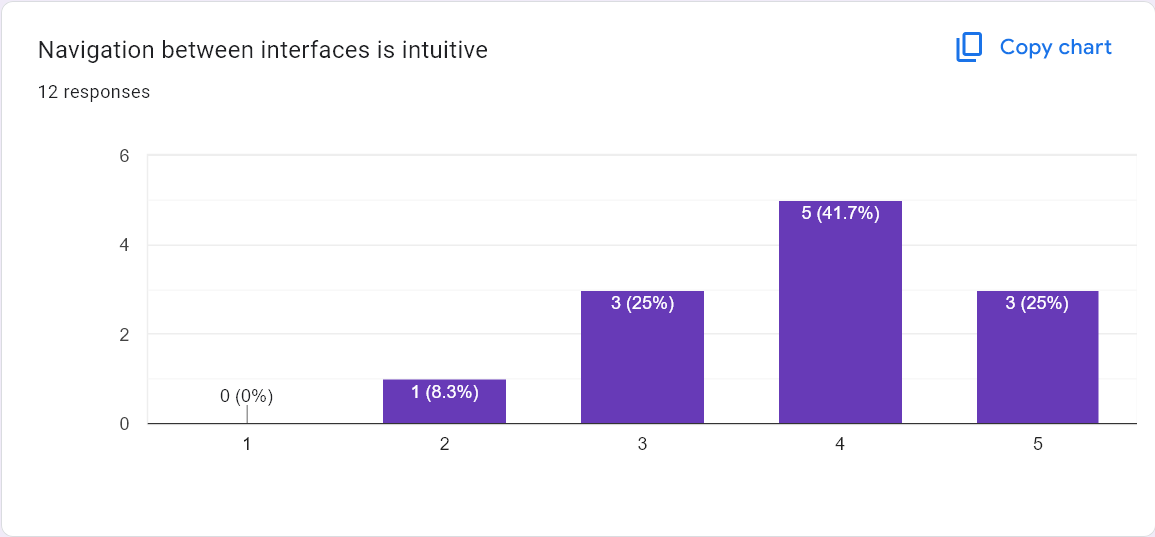
\includegraphics[scale=0.35]{./Images/Q1.png}}
  \label{fig:StraightForward}
\end{figure}

\begin{figure}[htbp]
  \caption{"Placing objects is easy" statement ratings}
  \centerline{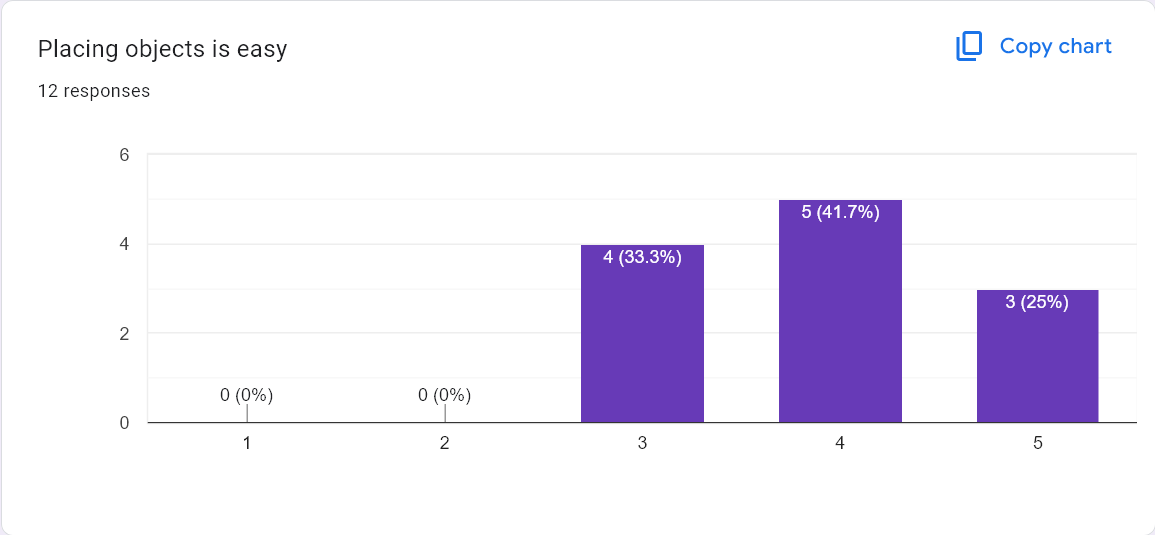
\includegraphics[scale=0.35]{./Images/Q2.png}}
  \label{fig:Navigation}
\end{figure}

\begin{figure}[htbp]
  \caption{"Generating objects is easy" statement ratings}
  \centerline{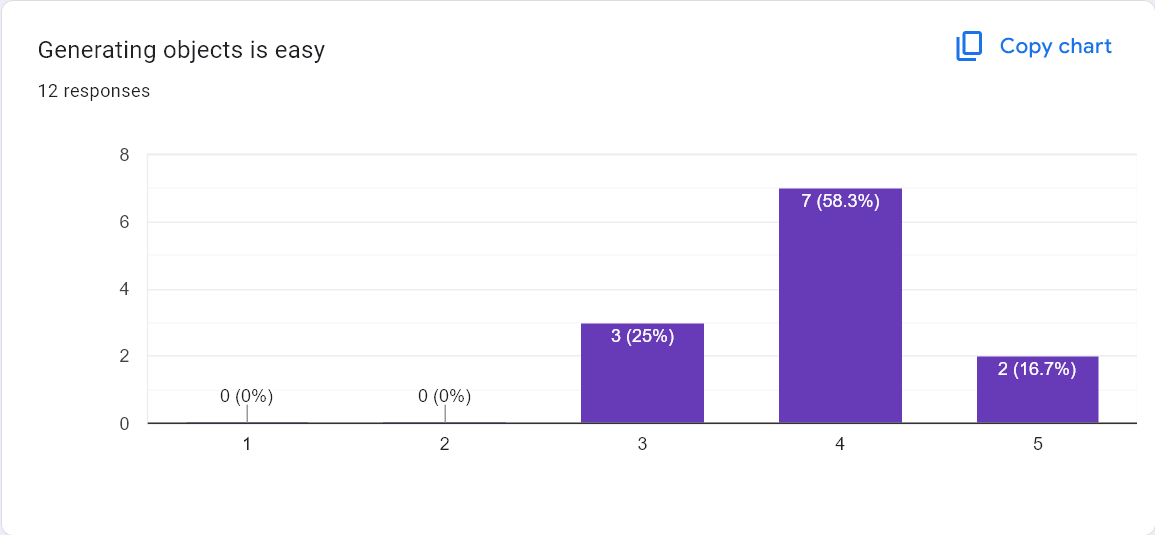
\includegraphics[scale=0.35]{./Images/Q3.png}}
  \label{fig:Detached}
\end{figure}

\begin{figure}[htbp]
  \caption{"It is easy to start a tour" statement ratings}
  \centerline{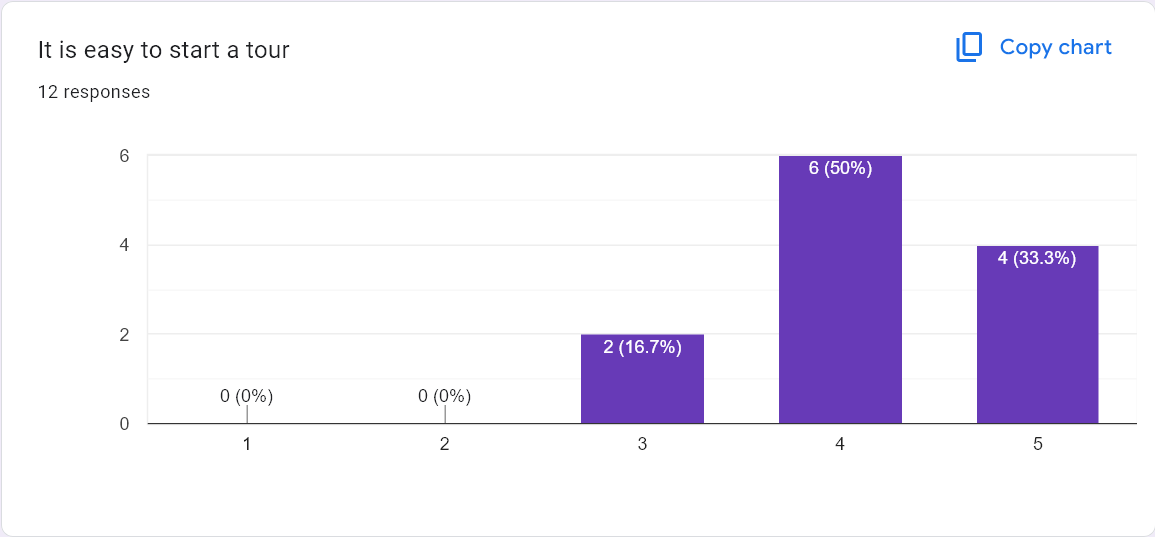
\includegraphics[scale=0.35]{./Images/Q4.png}}
  \label{fig:RealWorld}
\end{figure}

\begin{figure}[htbp]
  \caption{"Changing settings is easy" statement ratings}
  \centerline{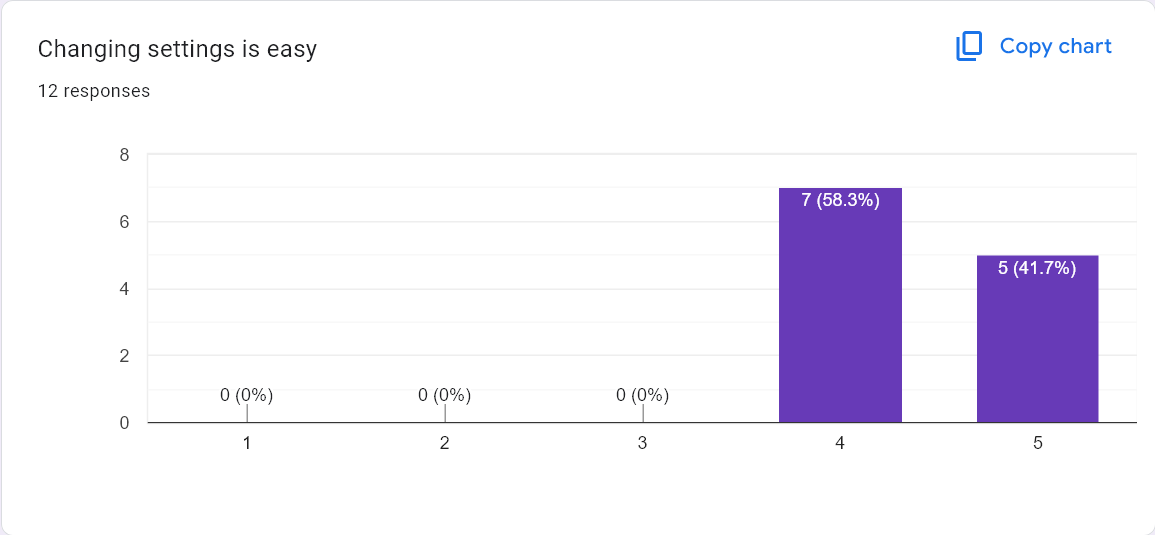
\includegraphics[scale=0.35]{./Images/Q5.png}}
  \label{fig:Fun}
\end{figure}

\begin{figure}[htbp]
  \caption{"The app is generally satisfying to use" statement ratings}
  \centerline{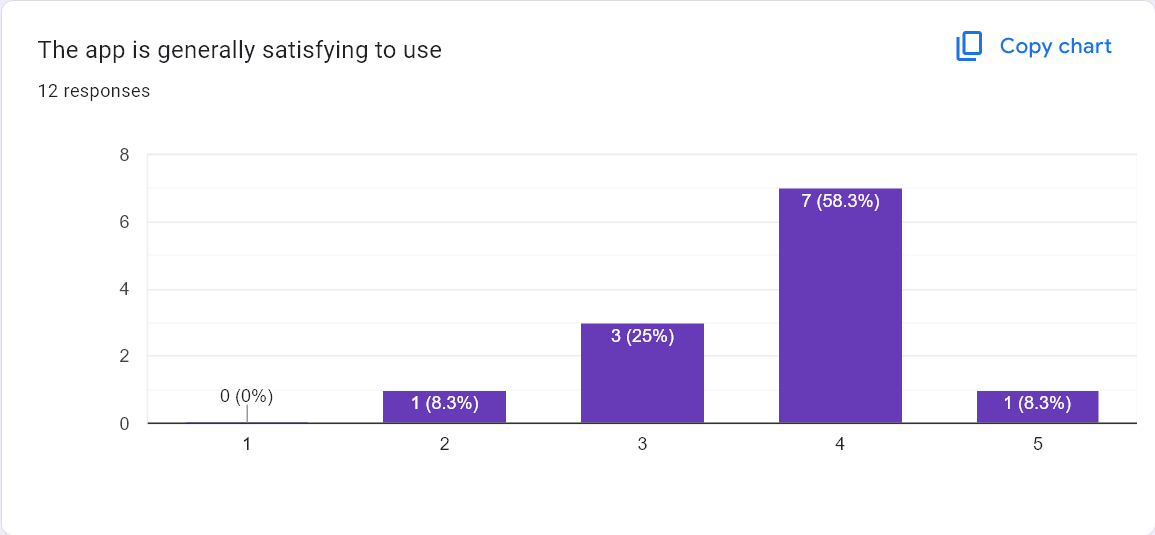
\includegraphics[scale=0.35]{./Images/Q6.png}}
  \label{fig:Social}
\end{figure}

\begin{figure}[htbp]
  \caption{"Using the app distracts from the surroundings" statement ratings}
  \centerline{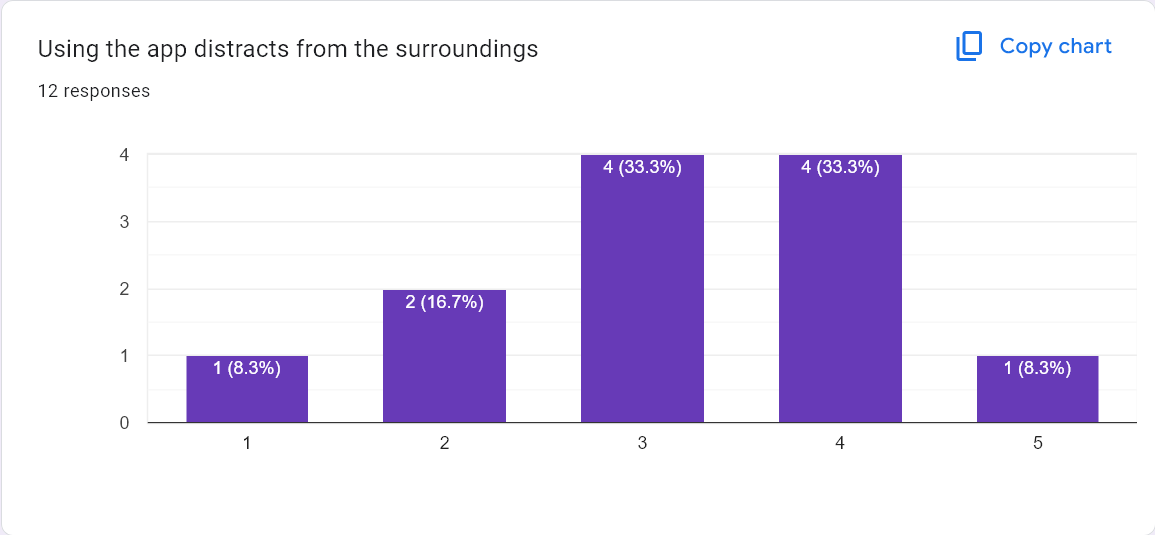
\includegraphics[scale=0.35]{./Images/Q7.png}}
  \label{fig:Enjoy}
\end{figure}

\newpage{}

\section*{Appendix --- Reflection}

The information in this section will be used to evaluate the team members on the
graduate attribute of Reflection.

The purpose of reflection questions is to give you a chance to assess your own
learning and that of your group as a whole, and to find ways to improve in the
future. Reflection is an important part of the learning process.  Reflection is
also an essential component of a successful software development process.  

Reflections are most interesting and useful when they're honest, even if the
stories they tell are imperfect. You will be marked based on your depth of
thought and analysis, and not based on the content of the reflections
themselves. Thus, for full marks we encourage you to answer openly and honestly
and to avoid simply writing ``what you think the evaluator wants to hear.''

Please answer the following questions.  Some questions can be answered on the
team level, but where appropriate, each team member should write their own
response:


\begin{enumerate}
  \item What went well while writing this deliverable?
  \item What pain points did you experience during this deliverable, and how
        did you resolve them?
  \item Which parts of this document stemmed from speaking to your client(s) or
        a proxy (e.g. your peers)? Which ones were not, and why?
  \item In what ways was the Verification and Validation (VnV) Plan different
        from the activities that were actually conducted for VnV?  If there were
        differences, what changes required the modification in the plan?  Why did
        these changes occur?  Would you be able to anticipate these changes in future
        projects?  If there weren't any differences, how was your team able to clearly
        predict a feasible amount of effort and the right tasks needed to build the
        evidence that demonstrates the required quality?  (It is expected that most
        teams will have had to deviate from their original VnV Plan.)
\end{enumerate}

\end{document}